\section{Sequence Labelling Tasks}
\label{sec:SeqTagging}

We evaluate the different word representations over four sequence
labelling tasks: POS-tagging (\pos), full-text chunking (\chunking) ,
NER (\ner) and MWE identification (\mwe). For
each task, we fed features into a first order linear-chain graph
transformer~\cite{collobert2011natural} made up of two layers: the upper
layer is identical to a linear-chain CRF~\cite{lafferty2001conditional},
and the lower layer consists of word representation and hand-crafted
features. If we treat word representations as fixed, the graph
transformer is a simple linear-chain CRF. On the other hand, if we can
treat the word representations as model parameters, the model is
equivalent to a neural network with word embeddings as the input
layer. We trained all models using AdaGrad~\cite{duchi2011adaptive}.


% \begin{figure}[t]
%   \centering
%   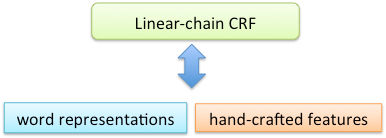
\includegraphics[scale = 0.3]{images/graph_transformer.png}
%   \caption{Architecture of linear-chain graph transformer}
%   \label{fig:graph_transformer}
% \end{figure}


As in~\newcite{turian2010word}, at each word position, we construct word
representation features from the words in a context window of size two
to either side of the target word, based on the pre-trained
representation of each word type.  For \brown, the features are the
prefix features extracted from word clusters in the same way
as~\newcite{turian2010word}. As a baseline (and to test \RQ[1]), we include a one-hot
representation (which is equivalent to a linear-chain CRF with only
lexical context features).

Our hand-crafted features for \pos, \chunking and \mwe, are those used
by \newcite{collobert2011natural}, \newcite{turian2010word}
and~\newcite{mwecorpus}, respectively. For \ner, we use the same feature
space as \newcite{turian2010word}, except for the previous two
predictions, because we want to evaluate all word representations with
the same type of model -- a first-order graph transformer.

In training the distributed word representations, we consider two
settings: (1) the word representations are fixed during sequence model
training; and (2) the graph transformer fine-tunes the token-level word
representations during training.


\begin{table*}
\begin{small}
\begin{tabular}{cccccc}
\hline
			& \textbf{Training} & \textbf{Development} & \textbf{\textit{In-domain} Test} & \textbf{\textit{Out-of-domain} Test} \\ \hline
\textbf{\pos} & \WSJ Sec.\ 0-18  & \WSJ Sec.\ 19--21 & \WSJ Sec.\ 22--24 & \EWT  \\
\textbf{\chunking} & \WSJ & \WSJ (1K sentences) & \WSJ (CoNLL-00 test) & \Brown \\
\textbf{\ner} & \Reuters (CoNLL-03 train) & \Reuters (CoNLL-03 dev) & \Reuters (CoNLL-03 test) & \MUC  \\
\textbf{\mwe} & \EWT (500 docs) & \EWT (100 docs)  & \EWT (123 docs) & --- \\
\hline
\end{tabular}
\caption{Training, development and test (in- and out-of-domain) data for each sequence labelling
  task.}
\label{datasplit}
\end{small}
\end{table*}


As outlined in \tabref{datasplit}, for each sequence labelling task, we
experiment over the de facto corpus, based on pre-existing
training--dev--test splits where available:\footnote{For the \mwe
  dataset, no such split pre-existed, so we constructed our own.}
\begin{compactenum}
\item[\textbf{\pos}:] the Wall Street Journal portion of the Penn
  Treebank (\newcite{Marcus:1993}: ``\WSJ'')
  with Penn POS tags
\item[\textbf{\chunking}:] the Wall Street Journal portion of the Penn
  Treebank (``\WSJ''),
  converted into IOB-style full-text chunks using the CoNLL conversion
  scripts for training and dev, and the WSJ-derived CoNLL-2000 full text chunking
  test data for testing \cite{TjongKimSang:Buchholz:2000}
\item[\textbf{\ner}:] the English portion of the CoNLL-2003 English Named Entity Recognition
  data set, for which the source data was taken from Reuters newswire
  articles (\newcite{TjongKimSang:DeMeulder:2003}: ``\Reuters'')
\item[\textbf{\mwe}:] the MWE dataset of \newcite{mwecorpus}, over a portion of text from the
  English Web Treebank\footnote{\url{https://catalog.ldc.upenn.edu/LDC2012T13}} (``\EWT'')
\end{compactenum}
 For all tasks other
than \mwe,\footnote{Unfortunately, there is no
  second domain which has been hand-tagged with MWEs using the method of
  \newcite{mwecorpus} to use as an out-of-domain test corpus.} we
additionally have an out-of-domain test set, in order to evaluate the
out-of-domain robustness of the different word representations, with and
without fine-tuning. These datasets are as follows:
\begin{compactenum}
\item[\textbf{\pos}:] the English Web Treebank with Penn POS tags (``\EWT'')
\item[\textbf{\chunking}:] the Brown Corpus portion of the Penn
  Treebank (``\Brown''), 
  converted into IOB-style full-text chunks using the CoNLL conversion
  scripts
\item[\textbf{\ner}:] the MUC-7 named entity recognition corpus\footnote{https://catalog.ldc.upenn.edu/LDC2001T02} (``\MUC'')
\end{compactenum}

For reproducibility, we tuned the hyperparameters with random search
over the development data for each task~\cite{bergstra2012random}. 
In this, we randomly sampled 50 distinct hyperparameter sets with the
same random seed for the non-updating models (i.e.\ the models that
don't update the word representation), and
sampled 100 distinct hyperparameter sets for the updating models (i.e.\
the models that do). 
For each set of hyperparameters and task, we train a model over its
training set and choose the best one based on its performance on development data~\cite{turian2010word}. 
We also tune the word representation hyperparameters -- namely, the word
vector size $d$ and context window size $m$ (distributed
representations), and in the case of \Brown, the number of clusters.

For the updating models, we found that the results over the test data
were always inferior to those that do not update the word
representations, due to the higher number of hyperparameters and small
sample size (i.e.\ 100).
Since the two-layer model of the graph transformer contains a distinct
set of hyperparameters for each layer, we reuse the best-performing
hyperparameter settings from the non-updating models, and only tune the
hyperparameters of AdaGrad for the word representation layer. 
This method requires only 32 additional runs and achieves consistently
better results than 100 random draws.

In order to test the impact of the volume of training data on the
different models (\RQ[3]), we split the training set into 10 partitions based on
a base-2 log scale (i.e., the second smallest partition will be twice
the size of the smallest partition), and created 10 successively larger
training sets by merging these partitions from the smallest one to the
largest one, and used each of these to train a model.
From these, we construct learning curves over each task.

For ease of comparison with previous results, we evaluate both
in- and out-of-domain using 
chunk/entity/expression-level F1-measure (``\fscore'') for all tasks except \pos,
for which we use token-level accuracy (``\accuracy'').
To test performance over OOV (unknown) tokens -- i.e., the words that do
not occur in the training set -- we use token-level accuracy for all
tasks (e.g.\ for \chunking, we evaluate whether the full IOB tag is
correct or not), due to the sparsity of all-OOV chunks/NEs/MWEs.

%\subsection{POS-tagging} We could choose one of the options. \subsubsection{Option 1} Almost the same setting as~\cite{collobert2011natural}, except adding one more test set.
% \noindent Training set: 0-18 of WSJ.
% \noindent Validation set: 19-21 of WSJ.
% \noindent Test set: 22-24 of WSJ, and English Web Treebank. We report model performances on these two test sets respectively.
% \noindent Feature space: the same set as in~\cite{collobert2011natural}

% \subsection{Chunking} The same setting as~\cite{turian2010word}\\
% \noindent Training set: WSJ train set.
% \noindent Validation set: Randomly sampled 1000 sentences from the train set for development.
% \noindent Test set: CoNLL2000 test set.
% \noindent Feature space: the same set as in~\cite{turian2010word}

% \subsection{MWE Identification} Training set: randomly sampled 500 documents from Nathana��s corpus. 
% \noindent Validation set: randomly sampled 100 documents from Nathana��s corpus.
% \noindent Test set: remaining 123 documents from Nathana��s corpus..
% \noindent Feature space: the same set as in~\cite{mwecorpus}

%\subsection{Named entity recognition} Training set: CoNLL03 train set.
% \noindent Validation set: CoNLL03 development set.
% \noindent Test set: CoNLL03 test set and MUC7. We report model performances on these two test sets respectively.
% \noindent Feature space: the same set as in~\cite{turian2010word}


%%% Local Variables: 
%%% mode: latex
%%% TeX-PDF-mode: t 
%%% TeX-master: "WordEmbEvaluation"
%%% End: 
